\documentclass[conference,letterpaper]{IEEEtran}
\usepackage{fontspec}
\setmainfont{texgyretermes}[Extension=.otf,UprightFont=*-regular,BoldFont=*-bold,ItalicFont=*-italic,BoldItalicFont=*-bolditalic]
\usepackage[spanish,es-noshorthands,es-tabla,es-nodecimaldot]{babel}
\usepackage{cite}
\usepackage{amsmath}
\usepackage{graphicx}
\usepackage{booktabs}
\usepackage{tikz}
\usetikzlibrary{positioning,arrows.meta}
\usepackage[hidelinks]{hyperref}
\graphicspath{{../figures/}}
\renewcommand{\IEEEkeywordsname}{Palabras clave}
\renewcommand{\IEEEbibitemsep}{0pt plus 0.5pt}

\begin{document}

\title{Predicción espacio-temporal del rendimiento de papa en los Andes peruanos: kriging espacio-temporal, Random Forest espacial y XGBoost con la ENA, PISCO y TerraClimate, 2015--2025}

\author{\IEEEauthorblockN{Danny Christian Lopez Pajsi}
\IEEEauthorblockA{\textit{Facultad de Ingeniería Estadística e Informática} \\
\textit{Universidad Nacional del Altiplano}\\
Puno, Perú \\
dannylopez@est.unap.edu.pe}}

\maketitle

\begin{abstract}
La papa sostiene la seguridad alimentaria de los Andes peruanos, pero su rendimiento depende de un clima cada vez más variable y de prácticas de manejo desiguales. Este estudio integra tres fuentes oficiales en una sola base a nivel distrito-año: la Encuesta Nacional Agropecuaria (ENA) 2015--2025, la precipitación PISCOp v2.1 y las temperaturas de TerraClimate v1.1. Se procesaron 3,8 millones de filas de la ENA, de las que se extrajeron 130\,098 registros de papa, junto con 2,8 millones de valores de lluvia y 51,2 millones de valores de temperatura; agregados por distrito y campaña, dieron 4\,919 observaciones de 978 distritos de la sierra con 20 predictores, con las que se compararon seis modelos de cuatro familias: una réplica del protocolo de Tamayo-Vera et al.\ (2025), con Random Forest y gradient boosting, como referencia; XGBoost con coordenadas y un Random Forest espacial con información de vecinos; kriging espacio-temporal con regresión; y un híbrido de Random Forest con kriging espacio-temporal de residuos. Se evaluaron con validación temporal, validación espacial por bloques y en la ronda 2025, no usada en ningún ajuste. El Random Forest espacial obtuvo el menor error en la validación temporal (RMSE de 2,96~t/ha; $R^2=0{,}41$) y en 2025 (RMSE de 2,79~t/ha; $R^2=0{,}53$), con reducciones de 5,9\,\% (IC 95\,\%: 3,9--7,8) y 9,2\,\% (IC 95\,\%: 5,3--13,0) frente a la réplica, con validación cruzada anidada. En distritos no observados ganó el híbrido con kriging (RMSE de 3,38~t/ha; $R^2=0{,}24$), mientras que los modelos basados en vecinos perdieron precisión. Los intervalos bootstrap de la mejora excluyeron el cero en los tres esquemas. Con el modelo elegido se predijo 2025 con intervalos de predicción conformales al 95\,\%, cuya cobertura empírica fue del 97,3\,\%. Los predictores más importantes fueron la fertilización, el tipo de papa y la superficie. Los resultados muestran que el desempeño depende del esquema de validación y que la validación espacial es indispensable al predecir rendimientos agrícolas.
\end{abstract}

\begin{IEEEkeywords}
rendimiento de papa, kriging espacio-temporal, Random Forest espacial, validación cruzada espacial, Encuesta Nacional Agropecuaria, PISCO
\end{IEEEkeywords}

\section{Introducción}
La papa es uno de los cultivos que más contribuye a la seguridad alimentaria mundial, en especial en países en desarrollo con altos niveles de pobreza y desnutrición \cite{devaux2020}. En la sierra del Perú la cultivan sobre todo pequeños productores de secano, cuya vulnerabilidad climática se agrava por estructuras sociopolíticas que no priorizan su protección \cite{highlands2021}. Los propios productores perciben que el clima ha cambiado y que su producción ha disminuido \cite{perception2025}.

Los estudios agronómicos confirman esa vulnerabilidad. En el Altiplano peruano, la reducción de la precipitación es el principal canal por el que el cambio climático afecta a la papa de secano \cite{aquacrop2024}. En los Andes centrales, la brecha de rendimiento de los pequeños productores promedia el 42\,\% del rendimiento potencial, y el nitrógeno inorgánico es su principal factor explicativo \cite{yieldgap2020}. Esto ha impulsado la búsqueda de variedades nativas tolerantes a la sequía \cite{landraces2023} y a las heladas \cite{frost2024}, y a escala nacional se ha examinado la influencia del clima regional en los rendimientos agrícolas \cite{peruyield2026}. Anticipar el rendimiento a nivel local es, por tanto, útil para focalizar asistencia, seguros y programas de adaptación.

El aprendizaje automático se ha convertido en la herramienta dominante para predecir rendimientos. Las revisiones sistemáticas identifican a Random Forest y a los métodos de gradient boosting como los algoritmos más usados, casi siempre con variables climáticas entre los predictores \cite{vanklompenburg2020,shawon2025,obahoundje2025,plants2025}. Random Forest superó a la regresión lineal en predicciones globales y regionales \cite{jeong2016}, se ha combinado con simulación de cultivos a escala de condado \cite{sajid2022} y se ha usado para estimar el efecto de la escasez de insumos sobre la producción mundial \cite{inputs2023}; los extremos cálidos y secos simultáneos, por su parte, reducen los rendimientos de los principales cultivos a escala global \cite{extremes2023}. En la papa, Random Forest y XGBoost predijeron el rendimiento a partir de imágenes de drones en la sierra central del Perú ($R^2>0{,}74$) \cite{ccopi2024}, Random Forest y gradient boosting lo hicieron en la sierra sur ($R^2=0{,}54$) \cite{uav2026sur}, y estos modelos se han comparado con redes profundas \cite{potato2024ml}. A escala regional, Tamayo-Vera et al.\ \cite{tamayovera2025} compararon once modelos con 58 variables de clima, suelo y NDVI para la Isla del Príncipe Eduardo (Canadá) y reportaron un $R^2$ de 0,99 con Random Forest.

Sin embargo, los datos de rendimiento tienen autocorrelación espacial: los distritos vecinos comparten clima, suelos y prácticas. Cuando la validación no respeta esa estructura, las métricas sobreestiman la capacidad de predecir en lugares no observados \cite{roberts2017,ploton2020}. Meyer et al.\ mostraron que se requieren validación y selección de predictores espaciales \cite{meyer2019}, delimitar el área de aplicabilidad de los modelos \cite{meyer2021} y evaluar con cuidado los mapas producidos con aprendizaje automático \cite{meyer2022}. Tamayo-Vera et al.\ \cite{tamayovera2025} validaron con una partición temporal, pero no evaluaron la predicción en unidades espaciales no vistas.

La geoestadística ofrece una alternativa que modela la dependencia espacial de forma explícita y cuantifica la incertidumbre de cada predicción. El kriging espacio-temporal está implementado en el paquete \texttt{gstat} \cite{graler2016}, y los enfoques híbridos combinan aprendizaje automático con kriging de residuos \cite{sensors2022} o incorporan la información espacial dentro del Random Forest, mediante coordenadas y distancias \cite{hengl2018} o mediante los valores observados en los vecinos más cercanos \cite{sekulic2020}. No se ha comparado estos enfoques con modelos de aprendizaje automático estándar para el rendimiento de cultivos andinos con datos de encuesta oficial.

Este trabajo llena ese vacío con tres contribuciones: (i) una base integrada a nivel distrito-año que une la ENA 2015--2025 \cite{inei_ena} con la precipitación PISCOp \cite{aybar2020} y la temperatura TerraClimate \cite{abatzoglou2018}; (ii) una comparación de seis modelos, incluida una réplica del protocolo de ese artículo, bajo validación temporal, espacial y fuera del tiempo, con la ronda 2025 aún no usada en la literatura; y (iii) la evaluación del desempeño en el año de sequía de 2023 y un mapa de la incertidumbre de la predicción.

\begin{figure*}[!t]
\centering
% Flujo metodológico: etapas y variables que intervienen en cada una
\begin{tikzpicture}[
  font=\scriptsize, node distance=1.1mm and 3.4mm,
  caja/.style={draw=black!45, rounded corners=1.2pt, align=left, inner sep=2.2pt, text width=#1, fill=black!3},
  caja/.default=3.05cm,
  etapa/.style={font=\scriptsize\bfseries, align=center, text width=3.1cm},
  flecha/.style={-{Stealth[length=1.6mm]}, draw=black!55, line width=0.5pt}]

% ---------------- 1. Fuentes
\node[etapa] (t1) {1. Fuentes};
\node[caja, below=1mm of t1] (ena) {\textbf{ENA 2015--2025} (INEI)\\ 3,8 M filas $\rightarrow$ 130\,098 registros de papa; prácticas; $w_i$};
\node[caja, below=of ena] (pisco) {\textbf{PISCOp v2.1} (SENAMHI)\\ lluvia mensual, 0,1°; 2,8 M valores};
\node[caja, below=of pisco] (terra) {\textbf{TerraClimate v1.1}\\ $T_{\min}$ y $T_{\max}$ mensual, 1/30°; 51,2 M valores};
\node[caja, below=of terra] (mapa) {\textbf{Mapa distrital} (IGN)\\ 1\,873 distritos, centroides};

% ---------------- 2. Procesamiento
\node[etapa, right=of t1] (t2) {2. Procesamiento};
\node[caja=3.3cm, below=1mm of t2] (rend) {\textbf{Rendimiento} $Y_{d,t}$ (t/ha): producción (P219) / superficie (P217), estimador de razón con $w_i$};
\node[caja=3.3cm, below=of rend] (man) {\textbf{Manejo} (10, proporciones ponderadas): superficie media, riego, semilla certificada, papa nativa, abono, fertilizante, plaguicida, asistencia técnica, capacitación, asociatividad};
\node[caja=3.3cm, below=of man] (cli) {\textbf{Clima por campaña} ago--jul (10): lluvia de campaña, siembra y crecimiento, anomalía, meses secos, $T_{\min}$, $T_{\max}$, amplitud, mínima más baja, meses con helada};

% ---------------- 3. Base integrada
\node[etapa, right=of t2] (t3) {3. Base integrada};
\node[caja=2.75cm, below=1mm of t3, fill=blue!6, draw=blue!45] (base) {\textbf{Distrito-año} (sierra, $\geq$5 productores)\\[1pt] 4\,919 observaciones\\ 978 distritos\\ $Y_{d,t}$ + 20 predictores\\ + coordenadas $(x,y)$\\[1pt] DuckDB};

% ---------------- 4. Modelos
\node[etapa, right=of t3] (t4) {4. Modelos};
\node[caja=2.75cm, below=1mm of t4] (ref) {\textbf{Referencia}: réplica RF y réplica GB \cite{tamayovera2025}};
\node[caja=2.75cm, below=of ref] (aa) {\textbf{Aprendizaje automático}: XGBoost, RF espacial};
\node[caja=2.75cm, below=of aa] (geo) {\textbf{Geoestadística}: kriging espacio-temporal (ET)};
\node[caja=2.75cm, below=of geo] (hib) {\textbf{Híbrido}: RF + kriging ET};

% ---------------- 5. Validación
\node[etapa, right=of t4] (t5) {5. Validación};
\node[caja=2.75cm, below=1mm of t5] (val) {\textbf{Temporal}: 5 pliegues pasado$\rightarrow$futuro\\[1pt] \textbf{Espacial}: 5 bloques de distritos\\[1pt] \textbf{Futuro}: 2015--2024 $\rightarrow$ 2025};
\node[caja=2.75cm, below=of val, fill=blue!6, draw=blue!45] (met) {RMSE, MAE, $R^2$; Wilcoxon pareada};

% ---------------- flechas
\draw[flecha] (ena.east) -- (rend.west);
\draw[flecha] (ena.east) -- (man.west);
\draw[flecha] (pisco.east) -- (cli.west);
\draw[flecha] (terra.east) -- (cli.west);
\draw[flecha] (mapa.east) -- (cli.west);
\draw[flecha] (rend.east) -- (base.west);
\draw[flecha] (man.east) -- (base.west);
\draw[flecha] (cli.east) -- (base.west);
\draw[flecha] (base.east) -- (ref.west);
\draw[flecha] (base.east) -- (aa.west);
\draw[flecha] (base.east) -- (geo.west);
\draw[flecha] (base.east) -- (hib.west);
\draw[flecha] (ref.east) -- (val.west);
\draw[flecha] (aa.east) -- (val.west);
\draw[flecha] (geo.east) -- (val.west);
\draw[flecha] (hib.east) -- (val.west);
\draw[flecha] (val.south) -- (met.north);
\end{tikzpicture}

\caption{Flujo metodológico del estudio y variables que intervienen en cada etapa.}
\label{fig:flujo}
\end{figure*}

\section{Datos y métodos}
La Fig.~\ref{fig:flujo} resume las cinco etapas del estudio y las variables que entran y salen de cada una.

\subsection{Fuentes e integración}
La ENA es una encuesta anual por muestreo del Instituto Nacional de Estadística e Informática, con factores de expansión, que registra para cada productor los cultivos cosechados, la superficie, la producción y las prácticas de manejo \cite{inei_ena}. Se usaron las rondas 2015 a 2025: en 2020 la encuesta no se levantó y la ronda 2014 no contiene producción ni superficie en el archivo publicado. En 2015 y 2018 la superficie cosechada no se publicó en hectáreas; se reconstruyó con el factor hectárea/unidad declarada de la misma parcela, procedimiento que reprodujo el 100\,\% de las hectáreas oficiales en 2016--2022.

La precipitación mensual proviene de PISCOp v2.1 (SENAMHI) \cite{aybar2020,senamhi_piscop} y las temperaturas, de TerraClimate v1.1 \cite{abatzoglou2018,terraclimate_v11}. Cada variable se promedió dentro de los distritos del mapa oficial \cite{hdx_codab}, ponderando por la fracción de celda incluida, y se agregó por campaña agrícola (agosto a julio). Las ventanas de crecimiento (noviembre--marzo) y de riesgo de helada (octubre--abril) siguen el calendario de la propia ENA: en la sierra, el 62\,\% de la papa se siembra en octubre--noviembre y el 57\,\% inicia su cosecha en abril--mayo.

La Tabla~\ref{tab:fuentes} resume el volumen de datos procesado en cada fuente.

\begin{table}[!t]
\caption{Fuentes y volumen de datos procesados}
\label{tab:fuentes}
\centering
\footnotesize
\setlength{\tabcolsep}{2.4pt}
\begin{tabular}{lrl}
\toprule
Fuente & Datos procesados & Aporte \\
\midrule
ENA 2014--2025 (INEI) & 3\,843\,598 filas$^{a}$ & rendimiento, 10 var. \\
\quad registros de papa válidos & 130\,098 & \\
PISCOp v2.1 (lluvia) & 2\,824\,847 valores & 5 var. \\
TerraClimate v1.1 (Tmín, Tmáx) & 51\,209\,856 valores & 5 var. \\
Mapa distrital (IGN) & 1\,873 distritos & coordenadas \\
\midrule
Base integrada (distrito-año) & 4\,919 $\times$ 21 & modelos \\
\bottomrule
\multicolumn{3}{l}{\scriptsize $^{a}$ 2014--2024, más 158\,747 filas del módulo de cultivos 2025.} \\
\end{tabular}
\end{table}

\subsection{Variable objetivo y predictores}
El rendimiento de cada distrito $d$ y año $t$ se estimó con un estimador de razón ponderado:
\begin{equation}
Y_{d,t}=\frac{\sum_{i} w_i\,P_i}{\sum_{i} w_i\,S_i}\,,
\end{equation}
donde $P_i$ es la producción en toneladas, $S_i$ la superficie cosechada en hectáreas y $w_i$ el factor de expansión de cada registro de papa. De las 130\,112 filas de papa se descartaron 14 con rendimiento fuera de 0,1--60~t/ha; las 130\,098 restantes se agregaron en 7\,584 distrito-año, de los que 4\,919 corresponden a 978 distritos de la sierra con al menos cinco productores (442 a 609 por año). La Tabla~\ref{tab:vars} describe la variable objetivo y los 20 predictores, diez de manejo y diez de clima, todos completos en todas las rondas. Las variables de manejo son proporciones ponderadas con $w_i$ de los productores de papa del distrito (la de papa nativa, ponderada por superficie).

\begin{table}[!t]
\caption{Variables del modelo: fuente, unidad y media (desviación estándar) en la base de modelado ($n=4\,919$ distrito-año)}
\label{tab:vars}
\centering
\footnotesize
\setlength{\tabcolsep}{3pt}
\begin{tabular}{llll}
\toprule
Variable & Fuente & Unidad & Media (DE) \\
\midrule
\multicolumn{4}{l}{\textit{Objetivo}} \\
Rendimiento de papa $Y_{d,t}$ & ENA P219, P217 & t/ha & 8,80 (4,00) \\
\midrule
\multicolumn{4}{l}{\textit{Manejo}} \\
Superficie media de papa & ENA P217 & ha & 0,19 (0,23) \\
Riego & ENA P212 & 0--1 & 0,34 (0,38) \\
Semilla certificada & ENA P214 & 0--1 & 0,01 (0,07) \\
Papa nativa o amarga & ENA P204 & 0--1 & 0,26 (0,37) \\
Abono orgánico & ENA P236 & 0--1 & 0,88 (0,23) \\
Fertilizante & ENA P238 & 0--1 & 0,60 (0,38) \\
Plaguicida & ENA P240 & 0--1 & 0,68 (0,34) \\
Asistencia técnica & ENA P704 & 0--1 & 0,04 (0,10) \\
Capacitación & ENA P701 & 0--1 & 0,10 (0,16) \\
Asociatividad & ENA P801 & 0--1 & 0,06 (0,13) \\
\midrule
\multicolumn{4}{l}{\textit{Clima (campaña agosto--julio)}} \\
Lluvia de la campaña & PISCOp & mm & 763 (356) \\
Lluvia de siembra (set--nov) & PISCOp & mm & 133 (94) \\
Lluvia de crecimiento (nov--mar) & PISCOp & mm & 571 (255) \\
Anomalía de lluvia & PISCOp & \% & 0,0 (18,6) \\
Meses secos (nov--mar) & PISCOp & meses & 0,45 (0,75) \\
$T_{\min}$ de crecimiento & TerraClimate & °C & 5,41 (3,13) \\
$T_{\max}$ de crecimiento & TerraClimate & °C & 14,09 (2,65) \\
Amplitud térmica & TerraClimate & °C & 8,67 (1,40) \\
$T_{\min}$ más baja (oct--abr) & TerraClimate & °C & 4,00 (3,46) \\
Meses con helada (oct--abr) & TerraClimate & meses & 0,39 (1,23) \\
\bottomrule
\end{tabular}
\end{table}

\subsection{Modelos}
Los seis modelos se agrupan en cuatro familias según cómo tratan la dependencia espacio-temporal (Tabla~\ref{tab:modelos}). En todos, los predictores se transformaron con Yeo-Johnson y se estandarizaron (las coordenadas solo se estandarizaron), con parámetros estimados en el entrenamiento de cada pliegue. Las réplicas reproducen el protocolo de \cite{tamayovera2025}, con Random Forest \cite{breiman2001} o gradient boosting \cite{chen2016} sobre las $K$ variables más correlacionadas con el rendimiento, y suponen observaciones independientes. XGBoost y el RF espacial aprenden la dependencia de forma implícita: el primero con las coordenadas $s$ del centroide y el segundo, siguiendo a \cite{sekulic2020}, con el rendimiento $y_k$ y la distancia $d_k$ de los cinco distritos de entrenamiento más cercanos en el mismo año o, si no está en entrenamiento, en el anterior más próximo. El kriging ET y el híbrido modelan la covarianza de forma explícita: ajustan una tendencia (lineal o Random Forest) y predicen sus residuos ($\hat\varepsilon_i$, o $\hat r_i$ fuera de bolsa) por kriging ordinario con los 50 vecinos espacio-temporales más cercanos. Los pesos $\lambda_i$ provienen de un variograma separable, exponencial y con pepita, ajustado en cada pliegue,
\begin{equation}
\gamma(h,u)=\sigma^2\left[1-\rho_s(h)\,\rho_t(u)\right],
\end{equation}
donde $h$ es la distancia, $u$ el rezago en años y $\rho_s$, $\rho_t$ son las correlaciones espacial y temporal \cite{graler2016}. Solo estos dos modelos entregan la varianza de cada predicción.

\begin{table}[!t]
\caption{Modelos comparados: ecuación de predicción e hiperparámetros elegidos ($m$: variables por división; $n$: tamaño mínimo de nodo; $M$: árboles; $p$: profundidad)}
\label{tab:modelos}
\centering
\footnotesize
\setlength{\tabcolsep}{2.4pt}
\begin{tabular}{lll}
\toprule
Modelo & Ecuación de predicción & Hiperparámetros \\
\midrule
\multicolumn{3}{l}{\textit{Referencia, sin información espacial}} \\
Réplica RF & $\hat y=\tfrac{1}{B}\sum_{b}T_b(\mathbf{x}_K)$ & $K{=}15$, $m{=}3$, $n{=}5$ \\
Réplica GB & $\hat y=\sum_{m}\eta f_m(\mathbf{x}_K)$ & $K{=}20$, $M{=}200$, $p{=}5$ \\
\multicolumn{3}{l}{\textit{Aprendizaje automático con información espacial}} \\
XGBoost & $\hat y=\sum_{m}\eta f_m(\mathbf{x},s)$ & $M{=}200$, $p{=}5$ \\
RF espacial & $\hat y=\tfrac{1}{B}\sum_{b}T_b(\mathbf{x},s,y_k,d_k)$ & $m{=}4$, $n{=}5$ \\
\multicolumn{3}{l}{\textit{Geoestadística}} \\
Kriging ET & $\hat y=\mathbf{x}^{\top}\hat{\boldsymbol\beta}+\sum_{i}\lambda_i\hat\varepsilon_i$ & por pliegue \\
\multicolumn{3}{l}{\textit{Híbrido}} \\
RF + kriging ET & $\hat y=\hat y_{RF}(\mathbf{x})+\sum_{i}\lambda_i\hat r_i$ & $m{=}4$, $n{=}5$ \\
\bottomrule
\end{tabular}
\end{table}

El análisis se hizo en R con \texttt{tidyverse} \cite{wickham2019}, \texttt{recipes} y \texttt{rsample} de \texttt{tidymodels} \cite{kuhn2022}, \texttt{spatialsample} \cite{spatialsample2021}, \texttt{ranger} \cite{wright2017}, \texttt{xgboost}, \texttt{gstat} \cite{pebesma2004,graler2016} y \texttt{performance} \cite{ludecke2021}.

\subsection{Esquemas de validación}
Todos los modelos se evaluaron con las mismas particiones. (i) \textit{Temporal}: cinco pliegues de pasado a futuro sobre 2015--2024, con años de prueba 2019, 2021, 2022, 2023 y 2024, como en \cite{tamayovera2025}. (ii) \textit{Espacial}: cinco bloques de distritos vecinos formados con k-medias sobre sus coordenadas, de modo que ningún distrito de prueba aparece en entrenamiento \cite{roberts2017,ploton2020}. (iii) \textit{Futuro}: entrenamiento con 2015--2024 y prueba con 2025, ronda que no se usó en ningún ajuste. En cada pliegue temporal y espacial, los hiperparámetros se eligieron por búsqueda en grilla con una validación temporal interna que usa solo los datos de entrenamiento de ese pliegue (validación cruzada anidada); para 2025, con la validación temporal de 2015--2024 ($B=500$ árboles; $\eta=0{,}05$). Se reportan el RMSE, el MAE y el $R^2$. La mejora frente a la réplica RF se acompaña de su IC del 95\,\% por bootstrap (2\,000 remuestreos de distritos), y la diferencia de errores absolutos se contrastó con la prueba de Wilcoxon pareada. La autocorrelación de los residuos de 2025 se midió con el índice de Moran (cinco vecinos, 999 permutaciones).

\subsection{Predicción con el mejor modelo e intervalos}
El mejor modelo se eligió por su RMSE en la validación temporal 2015--2024, sin usar 2025. Con él, entrenado en 2015--2024, se predijo cada distrito de 2025 con un intervalo de predicción al 95\,\%. Se usó regresión cuantílica conformalizada \cite{romano2019}: un bosque de regresión cuantílica \cite{meinshausen2006}, con los mismos predictores del RF espacial, estima los percentiles 2,5 y 97,5, y una corrección conformal \cite{lei2018,angelopoulos2023} los amplía hasta garantizar la cobertura. La corrección es el cuantil $\lceil (n+1)(1-\alpha) \rceil / n$ de los puntajes $E_i=\max(\hat q_{\mathrm{inf}}-y_i,\; y_i-\hat q_{\mathrm{sup}})$, calculados en los pliegues temporales ($n=2\,500$; $\alpha=0{,}05$).

\section{Resultados}

\subsection{Patrón espacial y estructura de dependencia}
Por departamento (Fig.~\ref{fig:area}a), Arequipa, Junín y Pasco tienen los rendimientos más altos (13,6--18,8~t/ha en promedio) y Lambayeque, Puno e Ica los más bajos (4,5--6,1~t/ha). La campaña 2023 fue la más seca del periodo: la anomalía de lluvia fue negativa en casi toda la sierra (Fig.~\ref{fig:area}b) y alcanzó $-45$\,\% en Juliaca; ese año Puno registró su menor rendimiento, 3,6~t/ha, frente a 4,9--7,7~t/ha en las demás rondas. El variograma de los residuos (Fig.~\ref{fig:vario}) mostró una pepita espacial del 46\,\% y un rango exponencial de 83~km (rango práctico cercano a 250~km). Los rezagos de uno a cuatro años casi se superponen y el rango temporal alcanzó el límite superior del ajuste, lo que indica una componente persistente de cada distrito.

\begin{figure}[!t]
\centering
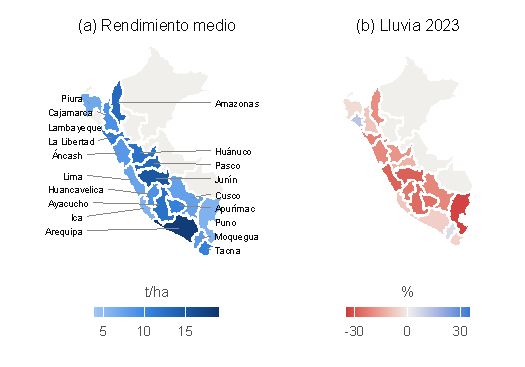
\includegraphics[width=\columnwidth]{fig1_area_estudio.pdf}
\caption{Papa de la sierra por departamento: (a) rendimiento medio 2015--2025 (estimador de razón con el factor de expansión); (b) anomalía de la lluvia de la campaña 2023, promedio de los distritos estudiados. En gris, departamentos sin papa de sierra.}
\label{fig:area}
\end{figure}

\begin{figure}[!t]
\centering
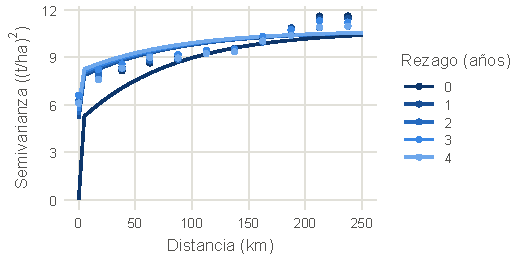
\includegraphics[width=\columnwidth]{fig2_variograma.pdf}
\caption{Variograma espacio-temporal empírico (puntos) y ajustado (líneas) de los residuos de la tendencia lineal, 2015--2024.}
\label{fig:vario}
\end{figure}

\subsection{Comparación de modelos}
La Tabla~\ref{tab:res} resume el desempeño. En la validación temporal, el RF espacial obtuvo el menor error (RMSE de 2,96~t/ha; $R^2=0{,}41$), 5,9\,\% menos que la réplica RF (IC 95\,\%: 3,9--7,8; $p=1\times10^{-10}$), y XGBoost quedó muy cerca. En la predicción de 2025 el orden se mantuvo: el RF espacial redujo el RMSE en 9,2\,\% (IC 95\,\%: 5,3--13,0; $R^2=0{,}53$ frente a 0,43; $p=7\times10^{-7}$). Sus residuos de 2025 mostraron poca autocorrelación espacial (I de Moran $=0{,}05$; $p=0{,}016$), un tercio de la de la réplica RF ($0{,}14$; $p=0{,}001$). En el año de sequía de 2023, su $R^2$ fue de 0,39 frente a 0,31 de la réplica.

La validación espacial cambió el orden y fue el escenario más difícil para todos los modelos. El híbrido RF + kriging ET obtuvo el menor error (RMSE de 3,38~t/ha; $R^2=0{,}24$), 3,3\,\% menos que la réplica (IC 95\,\%: 2,0--4,6), seguido del kriging ET, aunque la diferencia en el error absoluto típico no fue significativa (Wilcoxon $p=0{,}057$): la mejora proviene sobre todo de menos errores grandes. En cambio, el RF espacial y XGBoost con coordenadas tuvieron el peor desempeño ($R^2$ de 0,09 y 0,12), por debajo de la réplica, que no usa información espacial.

\begin{table}[!t]
\caption{Desempeño por esquema de validación con validación cruzada anidada (media de pliegues; RMSE en t/ha). En negrita, el mejor de cada columna.}
\label{tab:res}
\centering
\setlength{\tabcolsep}{3.2pt}
\begin{tabular}{lccccccc}
\toprule
 & \multicolumn{2}{c}{Temporal} & \multicolumn{2}{c}{Espacial} & \multicolumn{2}{c}{Futuro 2025} & 2023 \\
\cmidrule(lr){2-3}\cmidrule(lr){4-5}\cmidrule(lr){6-7}\cmidrule(lr){8-8}
Modelo & RMSE & $R^2$ & RMSE & $R^2$ & RMSE & $R^2$ & $R^2$ \\
\midrule
Réplica RF \cite{tamayovera2025} & 3,15 & 0,33 & 3,49 & 0,20 & 3,07 & 0,43 & 0,31 \\
Réplica GB \cite{tamayovera2025} & 3,21 & 0,31 & 3,46 & 0,19 & 3,13 & 0,41 & 0,25 \\
XGBoost & 2,97 & 0,41 & 3,67 & 0,12 & 2,94 & 0,48 & 0,35 \\
RF espacial & \textbf{2,96} & \textbf{0,41} & 3,66 & 0,09 & \textbf{2,79} & \textbf{0,53} & \textbf{0,39} \\
Kriging ET & 3,35 & 0,24 & 3,41 & 0,21 & 3,49 & 0,27 & 0,24 \\
RF + kriging ET & 3,12 & 0,34 & \textbf{3,38} & \textbf{0,24} & 3,13 & 0,41 & 0,36 \\
\bottomrule
\end{tabular}
\end{table}

\subsection{Predicción de 2025 con el mejor modelo}
El RF espacial fue el mejor modelo en la validación temporal y se usó para predecir 2025. La Tabla~\ref{tab:pred} muestra la predicción puntual y el intervalo al 95\,\% de doce distritos: los seis con más productores de papa fuera de Puno y los seis con más productores de Puno. En los doce, el rendimiento observado cayó dentro del intervalo. En los 585 distritos, la cobertura empírica fue del 97,3\,\% (nominal 95\,\%), frente al 96,2\,\% del bosque cuantílico sin conformalizar. Los intervalos son anchos (mediana de 11,7~t/ha), lo que refleja la variabilidad real del rendimiento distrital estimado con pocos productores.

\begin{table}[!t]
\caption{Predicción de 2025 con el RF espacial (t/ha): rendimiento observado, predicción puntual e intervalo de predicción conformal al 95\,\%; $n$: productores de papa encuestados en 2025}
\label{tab:pred}
\centering
\footnotesize
\setlength{\tabcolsep}{2.4pt}
\begin{tabular}{llrrrc}
\toprule
Departamento & Distrito & $n$ & Observado & Predicho & IP 95\,\% \\
\midrule
Huánuco & Panao & 75 & 12,50 & 12,73 & [5,21; 21,53] \\
Junín & Ulcumayo & 73 & 15,09 & 15,74 & [8,13; 24,83] \\
Ayacucho & Acocro & 72 & 15,95 & 13,59 & [5,41; 20,98] \\
Ayacucho & Vinchos & 72 & 14,60 & 9,04 & [3,06; 19,73] \\
Pasco & Paucartambo & 68 & 19,90 & 15,85 & [5,87; 24,19] \\
Ayacucho & Los Morochucos & 67 & 12,42 & 11,91 & [5,36; 18,52] \\
\midrule
Puno & Ilave & 155 & 7,21 & 7,57 & [3,13; 13,13] \\
Puno & Moho & 96 & 5,88 & 7,39 & [3,10; 12,30] \\
Puno & Ácora & 74 & 8,72 & 7,29 & [2,64; 13,37] \\
Puno & Rosaspata & 73 & 6,17 & 7,24 & [2,94; 12,34] \\
Puno & Zepita & 72 & 6,43 & 6,98 & [2,53; 11,22] \\
Puno & Taraco & 64 & 6,89 & 6,45 & [2,58; 10,61] \\
\bottomrule
\end{tabular}
\end{table}

\subsection{Mapas e importancia de las variables}
Resumido por departamento (Fig.~\ref{fig:mapas}), el RF espacial reprodujo el patrón observado en 2025, con los mayores rendimientos en Junín y Pasco y los menores en Piura y Puno, aunque subestimó a los departamentos más productivos (Junín: 15,6~t/ha observado frente a 13,8 predicho; Pasco: 14,4 frente a 12,2). Los intervalos de predicción fueron más anchos en Arequipa y Tacna (19,5 y 17,6~t/ha) y más estrechos en Puno (9,3~t/ha). En la importancia por permutación (Fig.~\ref{fig:imp}), los predictores más influyentes fueron la proporción de productores que fertilizan, la de papa nativa o amarga y la superficie media, seguidos de cinco variables climáticas: la lluvia de la campaña, la temperatura mínima más baja, la lluvia de crecimiento, la temperatura mínima de crecimiento y la lluvia de siembra.

\begin{figure}[!t]
\centering
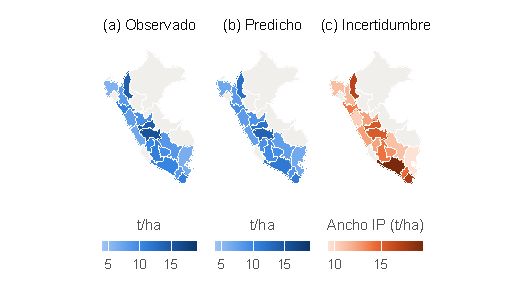
\includegraphics[width=\columnwidth]{fig4_mapas_2025.pdf}
\caption{Predicción de 2025 (ronda no usada en el ajuste) por departamento, promedio de los distritos ponderado por productores: (a) rendimiento observado; (b) predicho por el RF espacial entrenado con 2015--2024; (c) ancho medio del intervalo de predicción conformal al 95\,\%. Departamentos como en la Fig.~\ref{fig:area}.}
\label{fig:mapas}
\end{figure}

\begin{figure}[!t]
\centering
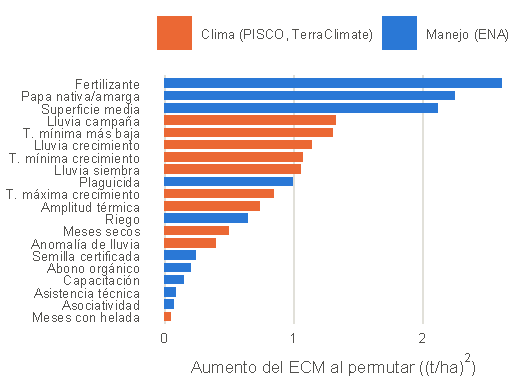
\includegraphics[width=\columnwidth]{fig5_importancia.pdf}
\caption{Importancia por permutación de los predictores en un Random Forest entrenado con 2015--2024.}
\label{fig:imp}
\end{figure}

\section{Discusión}
Los $R^2$ obtenidos (0,24 a 0,53 según el esquema) están muy por debajo del 0,99 de Tamayo-Vera et al.\ \cite{tamayovera2025}. En parte, la diferencia refleja los datos: rendimientos de una encuesta de pequeños productores, con pocos informantes por distrito y gran heterogeneidad de variedades y prácticas, frente a registros de una agricultura comercial homogénea. También refleja la validación: al replicar su protocolo con nuestros datos, la réplica RF alcanzó un $R^2$ de 0,33 en la validación temporal y de 0,20 en la espacial. Esta caída es moderada frente a la de Ploton et al.\ \cite{ploton2020}, cuyo modelo pasó de explicar más de la mitad de la variación con validación no espacial a un poder predictivo casi nulo con validación espacial, y coincide con las advertencias de Roberts et al.\ \cite{roberts2017} y de Meyer y Pebesma \cite{meyer2022}. Nuestro error en 2025 (RMSE de 2,79~t/ha) es comparable al de Random Forest con imágenes de drones en la sierra sur (RMSE de 2,72~t/ha; $R^2=0{,}54$) \cite{uav2026sur}, aunque aquí se predice a escala distrital y solo con datos de encuesta y clima.

El hallazgo central es que no hay un modelo superior en todos los esquemas. Cuando el objetivo es pronosticar distritos ya observados, los vecinos aportan información valiosa y el RF espacial, en la línea de \cite{sekulic2020,hengl2018}, fue el mejor. Cuando la zona de predicción carece de observaciones, esa información deja de existir y los modelos que dependen de ella o de las coordenadas extrapolan mal; allí el kriging de residuos, que modela la covarianza de forma explícita, fue más robusto. Esto concuerda con la recomendación de evaluar los modelos según la distancia a la que realmente se va a predecir \cite{linnenbrink2024} y de delimitar su área de aplicabilidad \cite{meyer2021}. Para un uso operativo, el modelo debe elegirse según el escenario: el RF espacial para pronosticar la próxima campaña en distritos encuestados, y el híbrido con kriging para estimar distritos sin muestra.

La importancia de la fertilización coincide con el hallazgo de que el nitrógeno inorgánico es el principal factor de la brecha de rendimiento de la papa en los Andes centrales \cite{yieldgap2020} y con que, a escala global, la falta de fertilizantes es el choque de insumos que causa las mayores pérdidas, de hasta 26\,\% en la producción de maíz \cite{inputs2023}. Así se responde a la limitación que señalan Tamayo-Vera et al.\ sobre la ausencia de variables de manejo \cite{tamayovera2025}. El peso de la lluvia de la campaña y de la temperatura mínima concuerda con los impactos de la menor precipitación en el Altiplano \cite{aquacrop2024}, con la relevancia de la tolerancia a la sequía \cite{landraces2023} y a las heladas \cite{frost2024}, y con el efecto negativo de los extremos cálidos y secos sobre los rendimientos \cite{extremes2023,plants2025}. La sequía de 2023 se tradujo en una caída abrupta del rendimiento en Puno, y el RF espacial mantuvo en ese año su ventaja sobre la réplica.

El estudio tiene limitaciones. Las temperaturas mensuales diluyen las heladas de pocas noches, lo que explica la baja importancia de los meses con helada; productos diarios como PISCOt \cite{pisco_t2023} permitirían índices más finos cuando cubran todo el periodo. El rendimiento distrital proviene de pocos productores en muchos distritos, lo que añade error de muestreo. Los residuos conservan una autocorrelación espacial débil pero significativa, que un modelo con efectos aleatorios espaciales podría absorber. Por último, el análisis es distrital y sus conclusiones no deben trasladarse al productor individual.

\section{Conclusiones}
Se construyó una base integrada de la ENA 2015--2025 con información climática de PISCOp y TerraClimate para predecir el rendimiento de papa en 978 distritos de la sierra peruana, y se compararon seis modelos de cuatro familias bajo validación temporal, espacial y fuera del tiempo. Los modelos con información espacial superaron a la réplica del protocolo de Tamayo-Vera et al.\ en los tres esquemas, con validación cruzada anidada e intervalos bootstrap de la mejora que excluyen el cero: el RF espacial redujo el RMSE en 5,9\,\% en la validación temporal y en 9,2\,\% en 2025, y el híbrido con kriging espacio-temporal lo redujo en 3,3\,\% en distritos no observados. Con el RF espacial se predijo 2025 con intervalos de predicción conformales cuya cobertura empírica fue del 97,3\,\%. El desempeño depende del esquema de validación, por lo que los estudios de predicción de rendimientos deberían reportar siempre una validación espacial. Como trabajo futuro se propone incorporar índices climáticos diarios, ponderar por el error de muestreo de cada distrito y extender el análisis a otros cultivos andinos.

\bibliographystyle{IEEEtran}
\bibliography{refs}

\end{document}
